%\documentclass[tikz,border=3mm]{standalone}
%\usetikzlibrary{calc}
%\usetikzlibrary{shapes, snakes, patterns, arrows}
%\begin{document}

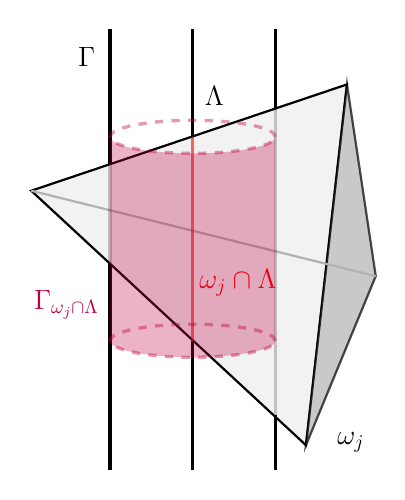
\begin{tikzpicture}[scale=0.7, every node/.style={scale=0.7}]
\pgfmathsetmacro{\factor}{1/sqrt(2)};


\coordinate  (A) at (-2.5,1.5,-2.1*\factor);
\coordinate  (B) at (3.8,4,0*\factor);
\coordinate  (C) at (3.6,-2,2*\factor);
\coordinate  (D) at (6.5,2.7,8*\factor);
\draw[thick, black,    fill=white!90!gray, opacity=1] (A) --(B)--(C)--cycle;
\draw[ thick,black,  fill=gray!60!, opacity=0.7] (D) --(B)--(C)--cycle;
\draw[thick,gray!60!] (D) --(A);
\node [font=\Large, right] at (3.5, -2.5) {$\omega_j $};


%cylinder Gamma
%\draw[dashed, very thick] (1, 5) ellipse (1.5 and 0.3);
%\draw[dashed, very thick] (1, -3) ellipse (1.5 and 0.3);
\draw[black, very  thick] (-0.5, 2.55) -- (-0.5, 5);
\draw[black, very thick, opacity=.2] (-0.5, 2.55) -- (-0.5, 0.75);
\draw[black, very  thick] (-0.5, 0.75) -- (-0.5, -3); 
\draw[ very thick] (2.5, 5) -- (2.5, 3.55);
\draw[ very thick, opacity =0.2] (2.5, 3.55) -- (2.5, -2);
\draw[very thick] (2.5, -2) -- (2.5, -3);
\node [font=\Large, right] at (-1.2, 4.5) {$\Gamma$};


%centerline \Lambda
\draw[very thick] (1, 5) -- (1, 3.05);
\draw[red, very thick, opacity=.6] (1, 3.05) -- (1, -0.65);
\draw[very thick, ]  (1, -0.65) -- (1, -3);
\node [font=\Large, right] at (1.1, 3.8) {$\Lambda$};
\node [font=\Large, right, red] at (1, 0.4) {$\omega _j \cap \Lambda$};

\draw[dashed, very thick, purple, opacity=.4] (1, 3.05) ellipse (1.5 and 0.3);
\draw[dashed, very thick, purple, opacity=.4] (1, -0.65) ellipse (1.5 and 0.3);

\fill [purple, opacity=0.3]  (-0.5, -0.65) arc (180:360:1.5 and 0.3) -- (2.5, 3.05) arc (0:180:1.5 and -0.3);
\node [font=\Large, right, purple] at (-2, 0) {$\Gamma_{\omega_j \cap \Lambda}$};

\end{tikzpicture}

%\end{document}